\section{Introduction}
\label{sec:intro}
Latent world models support state prediction, planning, and control~\citep{Ha2018}. They are commonly evaluated with a \emph{state probe}, a regressor fitted from encoded observations to physical states and applied to predicted latents~\citep{alain2016understanding,Anand2019AtariARI}. Its errors are in state units, so models with different latent spaces can be compared. The prediction horizon used for evaluation often extends far beyond the horizon supervised during training: Semigroup-JEPA probes $44$-step rollouts of predictors trained on one to five steps~\citep{Liu2026SemigroupJEPA}, and Koopman autoencoders trained on eight steps are decoded over a thousand~\citep{Azencot2020,nayak2024temporally}.

\begin{figure}[t]
\centering
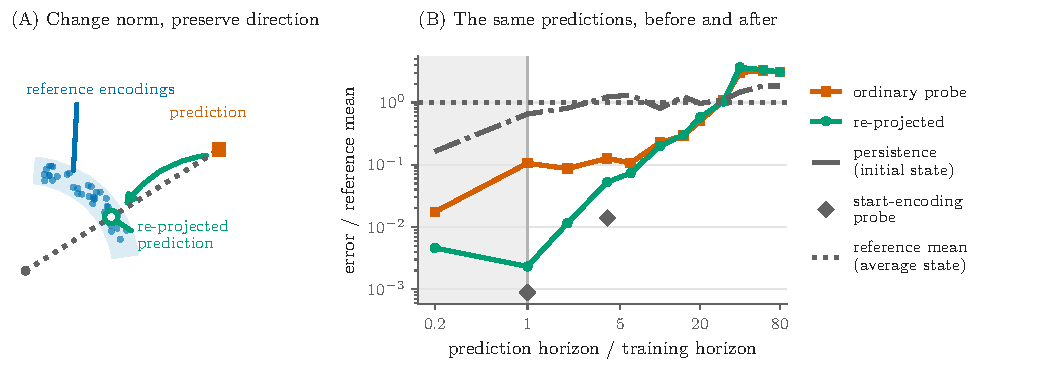
\includegraphics[width=\linewidth]{figures/fig_intro.pdf}
\caption{\textbf{Norm drift inflates the probe's error, and re-projection removes it.} \textbf{(A)} The prediction is moved along its existing direction to a reference radius estimated from observation encodings. \textbf{(B)} The same TCRL pendulum predictions are evaluated before and after this change. Errors are divided by the error of always predicting the mean state. Persistence predicts no change from the initial state. Shading marks the horizon supervised during training. Diamonds mark the start-encoding probe, fitted from the initial encoding to the state $T$ steps ahead. Longer horizons use separate rollouts under the same policy.}
\label{fig:intro}
\end{figure}

Each predicted latent becomes the input to the next step, so errors accumulate and predictions can move away from the encoded observations on which the probe was trained. The probe's error may then increase because the model predicts the wrong state, because the probe generalizes poorly to these unfamiliar inputs, or both. Testing the probe on held-out encodings does not distinguish these causes.

The simplest way for a prediction to move away from the encodings is in its norm. A latent state is a vector with a norm and a direction, and during autoregressive prediction errors in norm can accumulate while the direction stays accurate (Figure~\ref{fig:intro}B). A probe can change its output substantially in response to that norm change. Whether the model learns to control the norm depends on its training loss. TCRL uses a cosine loss that compares directions, ignoring the norm~\citep{zhao2023simplified}. TD-MPC2 and LeWorldModel use squared error, which also penalizes norm mismatch at supervised steps~\citep{Hansen2023,maes2026leworldmodel}. Beyond the training horizon, neither loss guarantees that prediction norms remain close to encoding norms.

Unlike an error in direction, an error in norm can be corrected without changing what the prediction encodes. Rescaling keeps the direction, and the encoder fixes the norm that a latent in that direction should have. We call this correction \emph{re-projection}: preserve the predicted direction, replace the norm with a reference radius estimated from encodings, and evaluate the same probe again (Figure~\ref{fig:intro}A). Because the direction and the rollout stay fixed, any change in the error is due to the norm. Re-projection splits the probe's error into the part the norm causes and a remainder that depends on the predicted direction. Current evaluations do not make this split.

%%BEGIN_INTRO_FINDINGS
We derive re-projection from the structure of the probe's error and test it on synthetic latents, on world models we train and on eleven published ones. For TCRL on pendulum, for example, re-projection removes $97$\% of the probe's error at the end of the training horizon (Figure~\ref{fig:intro}B). We make three contributions.
\begin{itemize}
\item We show that norm drift dominates the probe's error when training leaves the norm free. In cosine-trained world models whose dynamics do not constrain the norm, re-projection removes a median $99$\% of the error twenty steps ahead, while squared-error training and SimNorm keep the norm in check (Sections~\ref{sec:res_drift} and~\ref{sec:res_lewm}).
\item We show that norm drift reverses model rankings and that re-projection restores them. We build pairs of models whose true ranking is known and let the better model drift further. The ordinary probe ranks the worse model first in all $120$ pairs. The protocol confirms the true ranking in $88$ pairs. In the remaining $32$, where the two models differ least, the protocol reports the ranking as inconclusive, and it never confirms a wrong one (Section~\ref{sec:res_rank}).
\item We propose four checks that test whether a re-projected error can be used to compare models. In trained world models, they identify rollouts that do no better than a probe on the initial observation and rankings that change with the choice of probe (Section~\ref{sec:res_checks}).
\end{itemize}
%%END_INTRO_FINDINGS

\section{Related Work}
\label{sec:related}
\paragraph{World models and state probes.}
Decoder-based world models, including PlaNet, Dreamer, IRIS, and Koopman autoencoders, reconstruct observations and typically evaluate those reconstructions~\citep{Hafner2019Planet,hafner2020dream,Hafner2025,micheli2023transformers,Azencot2020}. Decoder-free models could fit an observation decoder after training, but are often evaluated with a state probe instead~\citep{Liu2026SemigroupJEPA,Radha2026UWMJEPA,terver2026what,zhou2025dinowmworldmodelspretrained}. A probe recovers selected physical quantities, avoiding the emphasis on visual detail in pixel errors~\citep{mathieu2016deep}. Because the probe is fitted on encodings of observed frames, it is accurate on a prediction only as long as the prediction resembles those encodings.

Decoder-free models commonly train their dynamics with a cosine loss, as in SPR, EfficientZero, and TCRL~\citep{Schwarzer2021SPR,ye2021mastering,zhao2023simplified}, or with squared error, as in TD-MPC2 and LeWorldModel~\citep{Hansen2023,maes2026leworldmodel}. The choice decides how freely the prediction norm can move. A cosine loss compares directions only and leaves the norm free to drift, while squared error penalizes a wrong norm. Even under squared error, a small error in norm compounds over a long rollout. The loss may compare raw latents or the outputs of a projection network, in which case a probe on the raw latents is applied to a representation that the loss does not supervise directly. Recursive prediction feeds model outputs back into the dynamics, so errors accumulate over the rollout~\citep{Talvitie2014,Kaiser2020,Janner2019}. Training on predicted inputs or on several future steps reduces this at the supervised horizons~\citep{Bengio2015ScheduledSampling,Venkatraman2015DaD,Lamb2016ProfessorForcing,Talvitie2017,Hafner2019Planet}, but beyond them the error keeps accumulating, and evaluations often go far beyond them. Output constraints such as SimNorm and min--max scaling bound the recurrent representation at every step~\citep{Hansen2023,Schrittwieser2020}. They are the only training choice that controls the norm at every horizon, but they confine each latent to a fixed range, such as the interval from zero to one, and so restrict the representation. A bound limits norm growth but need not keep predictions at the norms on which a probe was trained. Norm can also carry useful information, such as input familiarity or image quality~\citep{draganov2025norms,kim2022adaface}, so removing it calls for additional controls.

\paragraph{Probes on predicted latents.}
Several studies observe that predicted latents drift away from the encodings, in direction as well as in norm~\citep{ye2021mastering,wu2023slotformer,shah2026rollout}. One remedy is to fit the probe on predictions instead of encodings~\citep{Bear2021Physion,Nayebi2023MentalSim,Rao2026SkyJEPA,zheng2026contactguard}. Such a probe is accurate on predictions, but only at the horizons it was fitted on. ATM compares inverse-dynamics probes fitted on encoded and on predicted transitions~\citep{chen2026atm}. Other work measures the directional error and overshoot of predictions~\citep{vakalis2026intervention} or reports that rollout norms stay constant~\citep{sivasankar2026adaptive}. None of them measures how much of a probe's error the prediction norm causes.

Studies of representation probing show that conclusions depend on probe capacity and on suitable control tasks~\citep{alain2016understanding,Hewitt2019ControlTasks,Pimentel2020Probing,Voita2020MDL,Belinkov2022Probing}. Re-projection is a new kind of intervention on the probe's input, so it needs its own controls. We add controls for state information in the norm, for uninformative rollouts, and for directions far from the probe's training data, and use them to decide when the re-projected error can be trusted.

\section{Materials and Methods}
\label{sec:methods}
\subsection{Norm drift and state probes}
\label{sec:background}
\label{sec:formal_setup}
Let the world model's encoder $\phi$ map an observation $\mathbf o_t$ as $\z_t=\phi(\mathbf o_t)\in\mathbb R^D$. Given actions $\mathbf a_{t+k}$, the dynamics module $F_\theta$ produces a rollout
\begin{equation}
\hat{\z}_t=\z_t,\qquad
\hat{\z}_{t+k+1}=F_\theta(\hat{\z}_{t+k},\mathbf{a}_{t+k}).
\label{eq:recurrence}
\end{equation}
Here $\z_{t+k}$ is the encoding of the observed future frame and $\hat\z_{t+k}$ is its prediction. Training supervises steps $k\le H$. Evaluation may extend to $T>H$.

A state probe $r:\mathbb R^D\to\mathbb R^{d_y}$ is fitted on reference encodings with physical states $\mathbf y$ as targets and then applied to predictions. Its mean squared error over $n$ rollouts and $d_y$ state coordinates is
\begin{equation}
E_r(T)=\frac{1}{n d_y}\sum_{i=1}^{n}
\bigl\|r(\hat{\z}^{(i)}_{t+T})-\mathbf{y}^{(i)}_{t+T}\bigr\|^2 .
\label{eq:eval_error}
\end{equation}
We call $E_r$ the \emph{raw error} and measure how it changes when prediction norms are matched to those of reference encodings.

\subsubsection{Where the norm enters the error}
\label{sec:split}
We can rewrite a nonzero prediction as $\hat\z=\hat c\,\hat{\mathbf u}$, where $\hat c=\|\hat\z\|$ is its norm and $\hat{\mathbf u}=\hat\z/\|\hat\z\|$ is its unit direction. Let $\rho(\hat{\mathbf u})$ denote its \emph{reference radius}, the norm that encodings in direction $\hat{\mathbf u}$ have. When the encoder ends in a normalization, we compute the radius from that normalization, which gives the layer-normalization radius for our trained models and the exact SimNorm radius for TD-MPC2 (\supsec~\ref{app:radius}). Otherwise we take the norm of the reference encoding nearest in angle.

Re-projection replaces $\hat\z$ with $\tilde\z=\rho(\hat{\mathbf u})\hat{\mathbf u}$. The error of a single prediction, $r(\hat\z)-\mathbf y$, is the term inside the sum of Equation~(\ref{eq:eval_error}). Adding and subtracting the probe output at the reference radius splits it into two parts:
\begin{equation}
\begin{aligned}
r(\hat{\z})-\mathbf y &= r(\hat{\z})-\mathbf y-r(\tilde\z)+r(\tilde\z) \\
&=\underbrace{\bigl[r(\hat{\z})-r(\tilde\z)\bigr]}_{\text{change due to the norm}}+\underbrace{\bigl[r(\tilde\z)-\mathbf y\bigr]}_{\text{residual after rescaling}} .
\end{aligned}
\label{eq:probe_composition}
\end{equation}
The first term is the change caused by the norm. The second is the error remaining at the reference radius. It contains the error of the predicted direction together with any error the probe makes on directions unlike the encodings it was fitted on, and re-projection cannot reduce it.

\subsubsection{When the norm effect is large}
\label{sec:loss}
\label{sec:arch_constraint}
\label{sec:readout}
For a linear probe $r(\z)=W\z+\mathbf b$~\citep{alain2016understanding,Hewitt2019ControlTasks}, the norm effect factors into
\begin{equation}
r(\hat\z)-r(\tilde\z)
=\underbrace{\bigl(\hat c-\rho(\hat{\mathbf u})\bigr)}_{\text{norm mismatch}}\quad
\underbrace{W\hat{\mathbf u}}_{\text{scale sensitivity}} .
\label{eq:linear_norm_effect}
\end{equation}
The score therefore changes only when the predicted norm differs from its reference radius and the probe is sensitive to scale, that is, when $W\hat{\mathbf u}$ is not zero. Three factors decide how large these two terms are.
\begin{itemize}
\item \textbf{Training loss.} Cosine loss ignores the norm of the vector it compares. Squared error regulates the norm, but only at supervised steps. Neither guarantees matching norms throughout a rollout longer than the training horizon ($T>H$).
\item \textbf{Output constraints.} Explicit normalization can prevent norm mismatch at every step. SimNorm, for example, splits the latent into groups and applies a softmax within each group~\citep{Hansen2023}, so used on both encoder and dynamics it sets the norm of every prediction from its direction. A looser bound only limits growth and need not place predictions at the reference radius.
\item \textbf{Probe response.} Linear and ReLU probes give increasingly large outputs as the input norm grows~\citep{Hein2019ReLU,Xu2021Extrapolate}. A probe with bounded hidden activations, such as tanh, has bounded output. Normalizing the probe input removes scale sensitivity, but may discard information carried by norm.
\end{itemize}

Unless the design sets the norm of every prediction from its direction, as SimNorm on both encoder and dynamics does, or the probe normalizes its input, the size of the effect has to be measured.

\subsubsection{Measuring the effect of the norm}
\label{sec:reprojection}
At each horizon $T$, we evaluate the same fitted probe on raw and re-projected predictions, without changing the recurrent rollout. The re-projected error $E_r^{\mathrm{rep}}$ and its ratio to the raw error $E_r$ are
\begin{equation}
E_r^{\mathrm{rep}}(T)
=\frac{1}{n d_y}\sum_{i=1}^{n}
\bigl\|r(\tilde\z^{(i)}_{t+T})-\mathbf y^{(i)}_{t+T}\bigr\|^2,
\qquad
q_r(T)=\frac{E_r^{\mathrm{rep}}(T)}{E_r(T)} .
\label{eq:reprojection_factor}
\end{equation}
The \emph{re-projection factor} $q_r(T)$ is defined when $E_r(T)>0$. Values below one indicate that rescaling reduces error. For example, $q_r=0.1$ corresponds to a $90\%$ reduction. Values above one indicate increased error. The factor measures how much of the raw error the norm causes, while $E_r^{\mathrm{rep}}$ measures the error that remains under the same probe.

Re-projection can also discard information. The norm can itself carry state information, and under squared-error training, averaging uncertain future directions can shorten a prediction, so restoring its norm may increase error. Four checks test whether a re-projected error reflects state information.

\subsubsection{Checks}
\label{sec:checks}
\begin{itemize}
\item \textbf{Support check.} Re-projection restores the norm, but the probe is reliable on the re-projected prediction only if its direction lies among the encodings it was fitted on. Far from every encoding, the probe extrapolates, and its error no longer measures the model. We measure the angle of each prediction to the nearest reference encoding and call the prediction \emph{supported} when this angle lies below the 99th percentile of the same angles for held-out target encodings.
\item \textbf{Radius check.} We fit two probes on reference encodings, one on the direction alone and one on direction and norm. The gain in held-out $R^2$ shows how much state the norm carries that the direction lacks, and that re-projection would remove.
\item \textbf{Probe agreement.} A ranking of two models can depend on the choice of probe. We therefore order each pair with five probes (Section~\ref{sec:instruments}): the re-projected and the normalized probe, which ignore the norm, and the probe fitted on predictions, the neighbor probe and target retrieval, which do not extrapolate beyond the data they were fitted on.
\item \textbf{Null controls.} A useful prediction must beat predictors that need no learned dynamics.
\begin{itemize}
\item \emph{Persistence} applies the probe to the initial encoding, as if the state did not change, and the \emph{reference mean} always predicts the mean state of the reference data.
\item Random directions with the prediction norms, re-projected in the same way, show how much rescaling lowers the error when the direction carries no state.
\item Three null rollouts, with actions shuffled across episodes, with starts swapped across episodes, and with the untrained module, test whether the score reflects the episode's actions, its initial state, or anything learned.
\item A \emph{start-encoding probe}, fitted to predict the future state directly from the initial encoding, tests whether the rollout adds information beyond the initial encoding.
\end{itemize}
\end{itemize}

\subsubsection{The protocol}
\label{sec:decision}
The protocol applies these steps in order at every evaluated horizon, with the rollout and the fitted probe fixed (Table~\ref{tab:terms}). The probe is first checked on encodings, including the radius check. We then use the re-projection factor to choose between the raw and the re-projected error, the null controls to test whether that error reflects learned dynamics, and the support check and probe agreement to test whether a ranking holds. A ranking is \emph{confirmed} when it passes every step, \emph{rejected} when its models fail the null controls, and \emph{inconclusive} otherwise. \supsec~\ref{app:code} gives code for each step.

\begin{table}[tb]
\caption{The protocol at one horizon, with the rollout and the probe fixed. Step 3 compares medians over runs.}
\label{tab:terms}
\centering\footnotesize
\begin{tabular}{@{}l>{\raggedright\arraybackslash}p{0.25\linewidth}>{\raggedright\arraybackslash}p{0.27\linewidth}>{\raggedright\arraybackslash}p{0.3\linewidth}@{}}
\toprule
Step & Question & Quantity & Decision \\
\midrule
1. Probe on encodings & Is the probe accurate on encodings, and does the norm carry state? & Held-out $R^2$, scale sensitivity, radius gain & $R^2$ above $0.5$ required; radius gain above $0.05$: use the raw error \\
2. Re-projection & How much of the error does the norm cause? & Factor $q_r$, beside the probe's error on the encoded targets & $q_r$ below $0.9$: use the re-projected error; otherwise the raw error \\
3. Null controls & Does the prediction beat what needs no learned dynamics? & Re-projected error against persistence, reference mean, start-encoding probe, random directions and null rollouts & Any of them as good: model rejected, and so is a ranking that puts it first or pairs two rejected models \\
4. Support and probes & Does the probe extrapolate, and does a ranking depend on the probe? & Share of predictions supported, orderings under five probes & Re-projected and normalized probes agree, both models at least half supported and no probe reverses: confirmed; otherwise inconclusive \\
\bottomrule
\end{tabular}
\end{table}

\subsection{Experimental setup}
\label{sec:variants}
\label{sec:suite}
We test re-projection and the protocol in three settings of increasing realism: synthetic latents whose state content we control, world models we train ourselves while varying how their architecture, loss and constraints act on the norm, and eleven published world models.

\subsubsection{Synthetic latents}
Synthetic latents let us set the state that a latent encodes and its norm independently, so we know what a correct probe should report. Section~\ref{sec:res_suite} describes the constructions, and \supsec~\ref{app:synthetic} gives their details.

\subsubsection{Trained world models}
\label{sec:protocol}
The norm of a prediction depends on three design choices: the architecture of the dynamics module, the training loss, and constraints on the latent. We train world models on pendulum, cartpole and acrobot swing-up~\citep{Tassa2018} and vary each choice. Every model is trained to predict $H=6$ steps and evaluated on held-out episodes with random actions, five and twenty steps ahead. Reference episodes fit the probes, and separate scoring episodes measure prediction error (\supsec~\ref{app:impl}).

To test the architecture, we train four dynamics modules with the same cosine loss and data, ten runs per module and task, which gives $120$ base models. Non-Linear, a residual network, and Linear, a linear layer with additive action inputs, leave the norm free, so we expect their norms to drift. Linear-Penalized adds a penalty on the linear map's spectral radius, which discourages growth without preventing it. Orthogonal constrains the linear map to be orthogonal, so it preserves the norm before the action is added, and we expect little drift. Each model learns its own encoder with representation regularization~\citep{Bardes2022}, and the encoder ends in layer normalization, which gives the reference radius analytically (\supsec~\ref{app:radius}).

To test the loss, we replace the cosine loss with squared error, which penalizes norm mismatch at supervised steps, so we expect drift only beyond the training horizon. To test constraints, we rescale every predicted latent to the initial norm, apply SimNorm to encoder and dynamics, or remove the encoder's final normalization. The first two should remove the drift, and the last should keep it. Each of these four variants has five runs per module and task.

To test the probe where actions matter and all modules share one latent space, the shared-encoder variant trains only the dynamics of all four modules on the frozen encoder of one Non-Linear run per task, under random torques held for four frames, with ten runs per module and task, evaluated up to fifty steps ahead.

To test rankings whose true answer is known, we build models of known accuracy on the encoders of the thirty Non-Linear base models. Such a model predicts, for each scoring episode, the encoding of a real frame from another episode whose state lies at a chosen neighbor rank from the true state five steps ahead, so a lower rank gives a more accurate model. We let the more accurate model drift furthest from the reference radius, which should mislead the ordinary probe, and give every model ten seeds (\supsec~\ref{app:known}).

\subsubsection{Published world models}
\label{sec:lewm}
The trained models test one design choice at a time. To test whether norm drift distorts evaluations in practice, we apply the protocol to eleven published world models on sixteen tasks: TCRL~\citep{zhao2023simplified}, TD-MPC and TD-MPC2~\citep{hansen2022temporal,Hansen2023}, LeWorldModel~\citep{maes2026leworldmodel}, Semigroup-JEPA~\citep{Liu2026SemigroupJEPA}, plain and consistent Koopman autoencoders~\citep{Azencot2020}, KSL~\citep{mcinroe2021learning}, PlayVirtual~\citep{yu2021playvirtual}, and the MuZero, EfficientZero and Sampled EfficientZero checkpoints of LightZero~\citep{Schrittwieser2020,ye2021mastering,hubert2021learning,niu2023lightzero}. We use released checkpoints or the authors' code and settings (\supsec~\ref{app:published}), and train six of the models ourselves (\suptab~\ref{tab:fidelity}). For Koopman autoencoders and Semigroup-JEPA, we keep the authors' own decoder or probe, so that we test their evaluation as published. For the other models, we fit the same state probe as for our trained models, so that every model is evaluated with the same probe.

\subsubsection{Probes}
\label{sec:instruments}
Our main probe, the \emph{ordinary probe}, is a multilayer perceptron with one hidden layer of $64$ ReLU units, fitted on reference encodings with three random seeds (\supsec~\ref{app:encoder}). The \emph{re-projected probe} is the same fitted probe applied to re-projected predictions. To test whether a ranking depends on how the latents are read, we compare it with four other probes that either ignore the norm or cannot extrapolate: the \emph{normalized probe}, fitted on unit directions; a probe fitted on predictions; the \emph{neighbor probe}, which returns the mean state of the nearest reference encodings; and \emph{target retrieval}, the rank of the correct target among all encoded targets (\supsec~\ref{app:alternative_readouts}).

\subsubsection{Statistical analysis}
\label{sec:stats}
The base models and the shared-encoder variant have ten independent runs for each of the four modules (Non-Linear, Linear, Linear-Penalized and Orthogonal) and three tasks (pendulum, cartpole and acrobot), and the squared-error, fixed-radius, SimNorm and no-final-normalization variants have five. Errors compound multiplicatively over a rollout, so small differences between runs grow to orders of magnitude at long horizons, and we report medians over runs. To compare two models, we pair every run of one with every run of the other and take the share of pairs in which the first has the lower error. The first model is better when the $95$\% bootstrap interval of this share lies above one half.

%%BEGIN_RESULTS
\section{Results}
\label{sec:exp}
\subsection{Synthetic latents}
\label{sec:res_suite}
\begin{figure}[t]
\centering
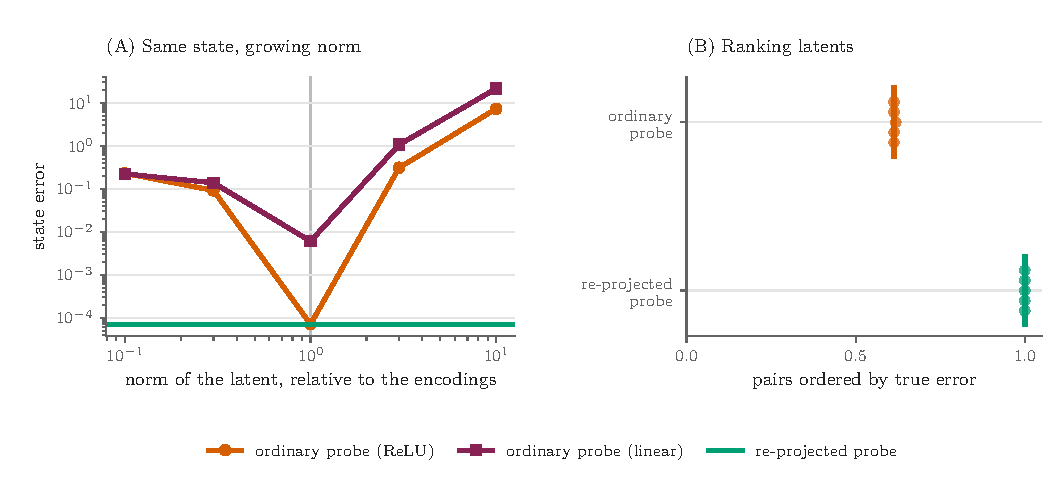
\includegraphics[width=\linewidth]{figures/fig_suite.pdf}
\caption{\textbf{Probes fail on synthetic latents whose norm drifts, and re-projection repairs them.} \textbf{(A)} Error of the ordinary probe, ReLU and linear, as the norm of a latent that stores the state in its direction grows or shrinks while the state stays the same; the re-projected probe returns to its error at the norm of the encodings. A norm that grows by $5$\% per prediction step reaches ten times its value after $47$ steps. \textbf{(B)} Share of pairs of latents that the ordinary and the re-projected probe order by their true state error, when the norm varies independently of that error; points are seeds, marks their means.}
\label{fig:suite}
\end{figure}
We first build latents whose content we control, to test whether re-projection resolves the problems of the ordinary probe identified in Section~\ref{sec:split}. Each latent stores a physical state in its direction, so a probe that reads the state correctly gives the same answer at any norm. We then change the norm and leave the state as it is, which is what autoregressive prediction does when it compounds a small error in norm. An error of $5$\% per step multiplies the norm by ten within $47$ steps. At that norm the ordinary probe's error is $27$ times that of always predicting the mean state, although the latent still encodes the state exactly, and the re-projected probe returns to its error at the original norm (Figure~\ref{fig:suite}A). When we give each latent a known state error and a norm chosen independently of it, the ordinary probe orders only about $61$\% of pairs of latents by their true error, where chance is 50\%, and the re-projected probe orders all of them (Figure~\ref{fig:suite}B). If the state is stored in the norm instead, re-projection would remove it, and the radius check detects this case before any correction (\supsec~\ref{app:synthetic}). On synthetic predictions for which we know which error is correct, or that neither is, the protocol decides correctly in $50$ of $50$ cases (\supsec~\ref{app:protocol_test}). Re-projection therefore removes the effect of the norm on both the error and the ranking of these latents, and the radius and support checks flag the cases in which it would mislead.

\subsection{Trained world models}
\label{sec:res_drift}
\begin{figure}[t]
\centering
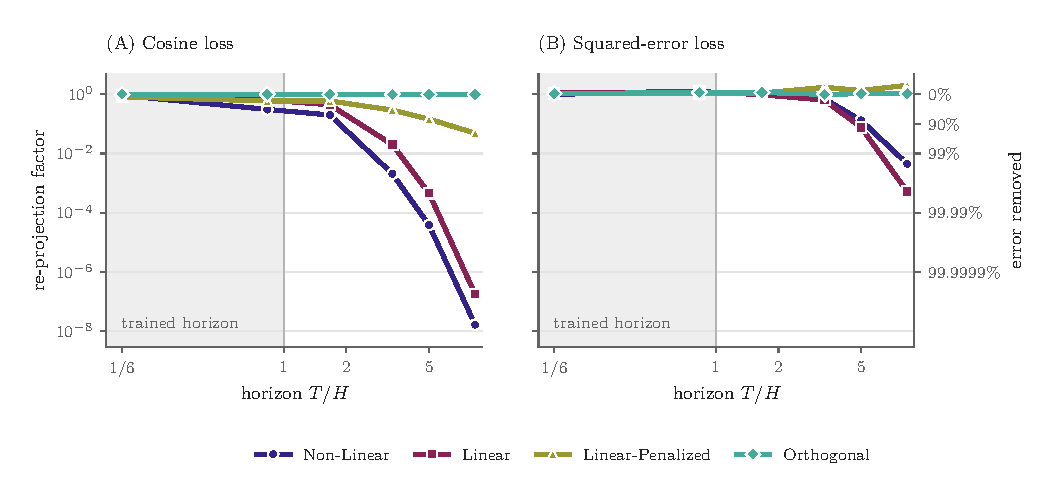
\includegraphics[width=\linewidth]{figures/fig_horizon.pdf}
\caption{Share of the probe's error that the norm causes in the trained modules under \textbf{(A)} the cosine and \textbf{(B)} the squared-error loss. Left axis: re-projection factor, the error after re-projection over the error before. Right axis: the share of the error that re-projection removes. Medians over runs and tasks. Shaded: trained horizon ($T\le H=6$).}
\label{fig:horizon}
\end{figure}

% Generated by scripts/cohort.py. Do not edit by hand.
\begin{table}[t]
\caption{What the ordinary probe and the re-projected probe report for the trained modules. Error: the error of the
modules that leave the norm free (Non-Linear and Linear) twenty steps ahead, over the error of always predicting the
mean state, medians over runs and tasks; bold, the error the protocol uses, re-projected when re-projection lowers
the error by more than a tenth. Ranking: the four modules ordered by each probe's median error twenty steps ahead,
best first (N Non-Linear, L Linear, P Linear-Penalized, O Orthogonal). Reversed: the module pairs, out of six, that the
two probes order differently five and twenty steps ahead. Each setting changes one component of the base models
(Section~\ref{sec:protocol}); \suptab~\ref{tab:arms_full} gives norms, factors and the radius check per task.}
\label{tab:arms}
\centering\footnotesize
\setlength{\tabcolsep}{5pt}
\begin{tabular}{@{}lrrcccrr@{}}
\toprule
 & \multicolumn{2}{c}{Error} & & \multicolumn{2}{c}{Ranking} & \multicolumn{2}{c}{Reversed} \\
\cmidrule(lr){2-3}\cmidrule(lr){5-6}\cmidrule(l){7-8}
Setting & Ordinary & Re-projected & & Ordinary & Re-projected & five & twenty \\
\midrule
\multicolumn{8}{@{}l}{\emph{norm free}} \\
\quad cosine loss & 458 & \textbf{\boldmath 2.47} & & O P L N & P N L O & 3 & 4 \\
\quad no final normalization & 376 & \textbf{\boldmath 2.10} & & O P N L & L P N O & 3 & 5 \\
\quad shared encoder & $1.6{\times}10^{4}$ & \textbf{\boldmath 1.29} & & O P L N & N L P O & 2 & 6 \\
\midrule
\multicolumn{8}{@{}l}{\emph{norm controlled}} \\
\quad squared-error loss & 9.15 & \textbf{\boldmath 6.29} & & P O L N & P O N L & 0 & 1 \\
\quad fixed radius & \textbf{\boldmath 2.13} & 2.11 & & P N L O & P N L O & 0 & 0 \\
\quad SimNorm & \textbf{\boldmath 1.39} & 1.46 & & O P L N & O P L N & 1 & 0 \\
\bottomrule
\end{tabular}
\end{table}


\paragraph{Free norms.}
Under cosine loss, twenty steps ahead, the ordinary probe reports an error $185$ times larger than that of the re-projected probe for the modules that leave the norm free (Table~\ref{tab:arms}). Per run, re-projection removes a median $99$\% of the ordinary probe's error (Figure~\ref{fig:horizon}A). Without the encoder's final normalization, the ordinary probe's error is $179$ times the re-projected one. With a shared encoder and actions that move the state, it is $1.3\times10^{4}$ times larger. Linear and ReLU probes respond to the norm in this way, while a tanh probe saturates, so its error stays bounded however far the norm drifts (\suptab~\ref{tab:v2_capacity}).

\paragraph{Rankings.}
The two probes also rank the modules differently, so they disagree on which model is better (Table~\ref{tab:arms}). Under cosine loss, Orthogonal comes first under the ordinary probe and last under the re-projected probe, because it keeps its norm while the other modules drift. Twenty steps ahead, the two probes disagree on four of the six module pairs under cosine loss, on five without final normalization, and on all six with a shared encoder. Sections~\ref{sec:res_rank} and~\ref{sec:res_checks} test whether such rankings hold, and on models of known accuracy re-projection ranks correctly where the ordinary probe fails.

\paragraph{Controlled norms.}
Where the design keeps the norm in check, both probes agree. Rescaling every predicted step to the initial norm gives $2.13$ under the ordinary probe and $2.11$ after re-projection, SimNorm $1.39$ and $1.46$, and in both settings the two probes rank the modules alike, up to one swap of neighbors. Squared-error training keeps norms close within the training horizon. There re-projection raises the error for ten of the twelve module--task combinations, because shorter predictions have less accurate directions, as expected when squared error averages over uncertain futures. The norm then carries the model's uncertainty, and the protocol keeps the raw error. Beyond the training horizon drift returns, with $9.2$ against $6.3$ twenty steps ahead (Figure~\ref{fig:horizon}B).

\subsection{Published world models}
\label{sec:res_lewm}
% Generated by scripts/published_table.py. Do not edit by hand.
\begin{table}[t]
\caption{What the ordinary probe and the re-projected probe report for published world models at $T^*$, the tested horizon where re-projection changes the error most: errors over the error of always predicting the mean state, medians over checkpoints. Reading: the protocol's conclusion from the re-projection factor, random directions with the predictions' norms, the mean state and the support check. $^\dagger$: the authors' own decoder or probe. $^r$: trained with the authors' code. \suptab~\ref{tab:published_full} gives every quantity, and \suptab~\ref{tab:published_more} the models whose loss compares projected latents.}
\label{tab:published}
\centering\footnotesize
\setlength{\tabcolsep}{4pt}
\begin{tabular}{@{}llrrrl@{}}
\toprule
Model & Task & $T^*/H$ & Ordinary & Re-projected & Reading \\
\midrule
TCRL$^r$ & pendulum & 1 & 0.11 & $2.3{\times}10^{-3}$ & norm hides an accurate prediction \\
TCRL$^r$ & cheetah-run & 80 & $9.1{\times}10^{3}$ & 1.18 & scale sensitivity only \\
TCRL$^r$ & four tasks & 60 & 6.16 & 2.42 & scale sensitivity only \\
Koopman AE$^\dagger$$^r$ & pendulum & 125 & $6.6{\times}10^{-3}$ & $6.4{\times}10^{-4}$ & inconclusive, unsupported \\
LeWorldModel & Two-Room & 1 & 0.02 & 0.01 & inconclusive, unsupported \\
TCRL$^r$ & three tasks & 30 & 1.22 & 1.17 & no correction needed \\
TD-MPC$^r$ & three tasks & 1 & 0.02 & 0.02 & no correction needed \\
TD-MPC2 (SimNorm) & three tasks & 133.3 & 2.75 & 2.75 & no correction needed \\
LeWorldModel & Push-T & 200 & 1.67 & 1.61 & no correction needed \\
Semigroup-JEPA, one-step$^\dagger$$^r$ & square & 9 & 0.67 & 0.62 & no correction needed \\
Semigroup-JEPA$^\dagger$$^r$ & square & 0.2 & 0.05 & 0.05 & no correction needed \\
\bottomrule
\end{tabular}
\end{table}


For TCRL on pendulum (Table~\ref{tab:published}), the ordinary probe reports $0.11$ of the mean state's error at the end of the training horizon, and re-projection lowers it to $2.3\times10^{-3}$. Assigning the predicted norms to the true target encodings reproduces the ordinary probe's error, so the predicted directions are accurate and the norm causes the ordinary probe's error (Figure~\ref{fig:intro}B; \supsec~\ref{app:problem}). For TCRL on cheetah-run, re-projection lowers the error from $9.1\times10^{3}$ to $1.2$ times the mean state's, but random directions with the same norms improve just as much, so the protocol attributes the reduction to the probe's sensitivity to scale. Random directions carry no state, so an improvement that they share says nothing about the predictions. For the Koopman autoencoders and for LeWorldModel on Two-Room, re-projection also lowers the error, but most predictions lie away from the encodings, and the protocol calls the reading inconclusive. A probe or decoder fitted on encodings extrapolates on such predictions, so neither its raw nor its re-projected error can be trusted there. For TD-MPC, TD-MPC2, LeWorldModel on Push-T and Semigroup-JEPA, both probes agree and no correction is needed. Each of these evaluations controls the norm. TD-MPC2 sets it with SimNorm, LeWorldModel bounds it with a normalized output head, TD-MPC is evaluated at the end of its training horizon, where squared error keeps it close, and the Semigroup-JEPA probe normalizes its input. KSL, PlayVirtual and LightZero apply their loss to the output of a projection network instead of the latent itself, so training never compares their raw predicted latents with the encodings. In raw latent space none of their predictions is supported, and the protocol calls the reading inconclusive. In the projection space, where the loss acts, the re-projected probe beats persistence and the mean state five steps ahead on every checkpoint (\suptab~\ref{tab:published_more}).

\subsection{Rankings with a known answer}
\label{sec:res_rank}
% Generated by scripts/known.py. Do not edit by hand.
\begin{table}[t]
\caption{Ranking models of known accuracy, five steps ahead. In each pair, the more accurate model drifts to three
times the reference radius and the other to half of that. Accuracy gap: how many times larger the less accurate
model's known state error is, median over encoders. Counts over the thirty trained encoders of the three tasks, with
ten seeds per model; for equally accurate models, any ordering is wrong. \suptab~\ref{tab:known_full} gives the
counts per task.}
\label{tab:known}
\centering\footnotesize
\setlength{\tabcolsep}{5pt}
\begin{tabular}{@{}lrrrcrrr@{}}
\toprule
 & \multicolumn{3}{c}{Ordinary probe} & & \multicolumn{3}{c}{Re-projection and checks} \\
\cmidrule(lr){2-4}\cmidrule(l){6-8}
Accuracy gap & right & wrong & open & & confirmed right & inconclusive & confirmed wrong \\
\midrule
equal & -- & \textbf{\boldmath 30} & 0 & & -- & 30 & 0 \\
1.67$\times$ & 0 & \textbf{\boldmath 30} & 0 & & 12 & 18 & 0 \\
3.32$\times$ & 0 & \textbf{\boldmath 30} & 0 & & 18 & 12 & 0 \\
5.40$\times$ & 0 & \textbf{\boldmath 30} & 0 & & 28 & 2 & 0 \\
15.2$\times$ & 0 & \textbf{\boldmath 30} & 0 & & 30 & 0 & 0 \\
\bottomrule
\end{tabular}
\end{table}


To test rankings against a known truth, we build models of known accuracy from the encoders of our trained models (Section~\ref{sec:protocol}). Each such model predicts the encoding of a real frame whose state lies close to the true future state, and the closer that frame, the more accurate the model. In every pair, the more accurate model also has the larger norm drift. The ordinary probe ranks the worse model first in all $120$ of these pairs (Table~\ref{tab:known}). For the $30$ pairs of equally accurate models, it declares one of the two better every time. The protocol confirms the true ranking in $88$ pairs, including all $30$ at the largest accuracy gap. For the other $32$, where the two models differ least, it reports the ranking as inconclusive, and it never confirms a wrong one. These pairs are most frequent on cartpole and acrobot, where the probe's error is larger even on the true encodings, so small differences between models fall within it.

\subsection{What the checks add}
\label{sec:res_checks}
\label{sec:consequences}
A lower re-projected error means that the norm distorted the score, but the model may still predict poorly. The checks detect two such cases in our trained modules. On pendulum and acrobot, re-projection makes the rollouts look accurate, but the start-encoding probe does at least as well (\suptab~\ref{tab:controls}). A ranking of these modules then says nothing about their dynamics, and the protocol rejects it. On cartpole the rollouts beat every null control, but the ordinary probe is inaccurate on their directions, while a probe fitted on the predictions has a much lower error. The support check flags the predictions that lie away from the encodings, and the protocol calls the cartpole rankings inconclusive. The same holds with a shared encoder up to fifty steps ahead, and no choice of thresholds confirms any of these rankings (\suptabs~\ref{tab:verdicts} and~\ref{tab:sensitivity}).
%%END_RESULTS

\section{Discussion}
\label{sec:discussion}
\subsection{Implications for evaluating world models}
%%BEGIN_SURVEY
Probe scores on predicted latents are routinely reported without the norm. Of $39$ evaluations of predicted latents that we surveyed, only one reports prediction norms, and three more report a related drift statistic. Seven apply a probe or decoder fitted on encodings to predictions beyond five times the training horizon, without input normalization or reported prediction norms (\supsec~\ref{app:literature}).
%%END_SURVEY

Where training leaves the norm free, the raw error of a linear or ReLU probe mostly measures the norm, and a better model can rank below a worse one with smaller norms. Re-projection removes this distortion without retraining, and its factor shows how much of a score the norm caused. We therefore recommend reporting prediction norms and the re-projection factor beside every probe score. The re-projected error should be used when the factor is below $0.9$ and the norm carries no state, and the raw error otherwise, as within the training horizon of squared-error models. Before ranking models, their rollouts should also be compared with the start-encoding probe and with rollouts under shuffled actions. We release a Python implementation of the protocol on GitHub (Data Availability Statement). From reference encodings with their states and predictions with their true states, it runs all four steps for a model and decides whether a ranking of two models is confirmed, inconclusive or rejected.

A probe fitted on encodings is unreliable on predictions whose direction lies away from every encoding, so an evaluation needs the option to call a ranking inconclusive. For a model evaluated through its own decoder, the raw error remains the measure of the complete system, because controlling the norm is part of that model's task.

\subsection{Limitations and future directions}
\label{sec:limitations}
\label{sec:future}
Our controlled experiments cover three environments and one encoder family. The support threshold comes from the targets' own distances to the reference encodings, so it is strict where those encodings lie densely. The same question arises wherever a probe or decoder fitted on encodings is applied to predictions, including the decoders of video world models and reward heads fitted on encoded states and queried along imagined rollouts. Applying the protocol to the evaluations our survey flags, and to real-robot and real-video data, would show how often norm drift distorts evaluations in practice.

\section{Conclusion}
\label{sec:conclusion}
%%BEGIN_CONCLUSION
Norm drift can dominate the error of a state probe on the predictions of a latent world model. Re-projection removes this error without retraining and restores the rankings that norm drift reverses, and four checks show when the re-projected error can be used to compare models. In cosine-trained world models that leave the norm free, it removed a median $99$\% of the probe's error twenty steps ahead. On models of known accuracy, it recovered $88$ of $120$ rankings that the ordinary probe had reversed, without a false confirmation. In our trained world models, the checks showed that none of the module rankings holds, because the rollouts did no better than the start-encoding probe or lay away from the encodings. We recommend reporting prediction norms and the re-projected error with every probe-based evaluation of predicted latents.
%%END_CONCLUSION
